%%%%%%%%%%%%%%%%%%%%%%%%%%%%%%%%%%%%
% Configuración general de página
%%%%%%%%%%%%%%%%%%%%%%%%%%%%%%%%%%%%
\documentclass[10pt,a4paper]{article}
\textheight = 21cm
\textwidth = 15cm
\topmargin = -0.5 cm
\oddsidemargin = 1cm

%%%%%%%%%%%%%%%%%%%%%%%%%%%%%%%%%%%%
% Paquetes
%%%%%%%%%%%%%%%%%%%%%%%%%%%%%%%%%%%%
\usepackage{amsmath}
\usepackage[utf8]{inputenx} % Permite introducir caracteres no ASCII
\usepackage[spanish]{babel} % Hace que los títulos aparezcan en español
\usepackage[pdftex]{graphicx} % uso de graficos en general
\usepackage{subcaption} % poder poner dos graficos como parte de uno
\usepackage{fancyhdr} % encabezado diferente para pag pares e impares
\usepackage{enumerate} % Permite crear listas
\usepackage{adjustbox}
\usepackage{tabu}
\usepackage{multicol} % Permite combinar columnas
\usepackage{multirow} % Permite combinar filas
\usepackage{colortbl} % Colorear celdas
\usepackage{booktabs} % Bordes en tablas
\usepackage{float} % Tablas y figuras flotantes
\usepackage[tablename=Tabla]{caption} % Permite insertar pies de figuras y títulos de tabla
\usepackage{etoolbox} % Permite arreglar errores de ciertos comandos
\usepackage[svgnames, table]{xcolor} % Colores a usar
\usepackage{footnote} % Notas al pie
\makesavenoteenv{tabular} % Permite insertar notas al pie en tablas
\usepackage[colorlinks=true, linkcolor=black, citecolor=black, urlcolor=cyan]{hyperref} % Permite insertar hyperlinks
\usepackage{url} % Corrige errores causados por la presencia de \, _ y otros caracteres en URLs

%%%%%%%%%%%%%%%%%%%%%%%%%%%%%%%%%%%%
% Configuración del formato del doc.
%%%%%%%%%%%%%%%%%%%%%%%%%%%%%%%%%%%%
\patchcmd{\thebibliography}{\section*{\refname}}{}{}{} % Inserta las referencias sin título
\apptocmd{\sloppy}{\hbadness 10000\relax}{}{} % Evita un warning molesto en la bibliografía
\captionsetup{hypcap=false} % Corrige un warning molesto al utilizar hyperref
%\AtBeginDocument{
%  \let\oldref\ref
%  \def\ref{\oldref*}} % Evita la creación de links en donde se llame al comando \ref
\graphicspath{{figuras/}} % Ubicación de los gráficos
\newcommand{\HRule}{\rule{\linewidth}{0.5mm}}
\DeclareGraphicsExtensions{.png,.jpg,.jpeg} % extensiones de las imágenes
\setlength{\parindent}{0.25in}

%%%%%%%%%%%%%%%%%%%%%%%%%%%%%%%%%%%%
% Incluimos el contenido
%%%%%%%%%%%%%%%%%%%%%%%%%%%%%%%%%%%%
\begin{document}

% Title
\begin{center}


\includegraphics[scale=0.1]{figures/itba_logo}
\vspace{1cm}

\textsc{\LARGE PAIByB - 16.85}\\[0.2cm]
\textsc{\Large Instituto Tecnológico de Buenos Aires}\\[0.2cm]
\vspace{1cm}

\HRule \\[0.2cm]
{ \huge \bfseries  ESTIMACIÓN DE RUIDO Y DENOISING \\[0.2cm] }
\HRule \\[1cm]

\vspace{1cm}

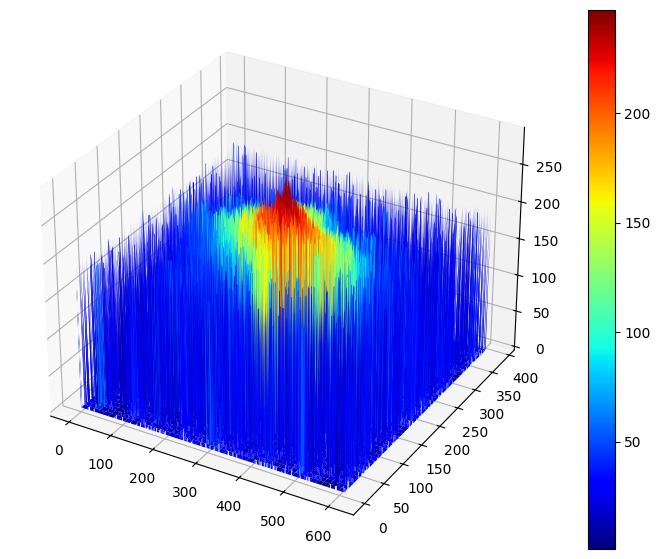
\includegraphics[width=0.5\linewidth]{figures/caratula}


\vspace{1cm}
\begin{multicols}{2}

% Author and supervisor
%\large
\begin{tabular}{l l}
  \emph{Profesor:}   &  Roberto Sebastián Tomás \\
\end{tabular}


% Integrantes
\columnbreak

%\normalsize
\begin{tabular}{l l}
  \emph{Alumnos:}   &  Lucas Neira \\
                    &  Ivo Bajlec \\
                    &  Gonzalo Grau \\
\end{tabular}

\end{multicols}
\vspace{1cm}

\textbf{Fecha de entrega}: 02/09/2024

\end{center}


%%%%%%%%%%%%%%%%%%%%%%%%%%%%%%%%%%%%%%%%
%                ENCABEZADO
%%%%%%%%%%%%%%%%%%%%%%%%%%%%%%%%%%%%%%%%
\thispagestyle{empty}
\pagestyle{fancy}
\headheight=60pt 	%para cambiar el tamaño del encabezado
\fancyhead[L]{PAIByB - 16.85 - 20242C}
\fancyhead[C]{\textbf{ITBA}}
\fancyhead[R]{TP1}

\newpage
\tableofcontents
\newpage
\section{Introducción} \label{sec:introduccion}
\section{Estimación de ruido} \label{sec:estimacion}

\subsection{Estimación estadística} \label{subsec:est_stat}

\subsection{Estimación por histograma} \label{subsec:est_hist}

\subsection{Estimación por Fourier} \label{subsec:est_fourier}

\subsection{Estimación por Wavelets} \label{subsec:est_wavelets}
\section{Denoising} \label{sec:denoising}

\subsection{Denoising espacial} \label{subsec:denoising_esp}

\subsection{Denoising por Fourier} \label{subsec:denoising_fourier}

\subsection{Denoising por Wavelets} \label{subsec:denoising_wav}

\subsection{Denoising por ecualización del histograma} \label{subsec:clahe}

\section{Discusión} \label{sec:discusion}


\section{Conclusión} \label{sec:conclusion}
\section{Anexos} \label{sec:anexos}
\newpage
\section*{Referencias}
\bibliographystyle{IEEEtran}
\nocite{*}
\bibliography{references}

\end{document}